\section{Results}

% ------------------------------------------------------------------------------
\begin{frame}{Layer \ding{172}: LLM and decision models lead, static tools trail}
  \centering
  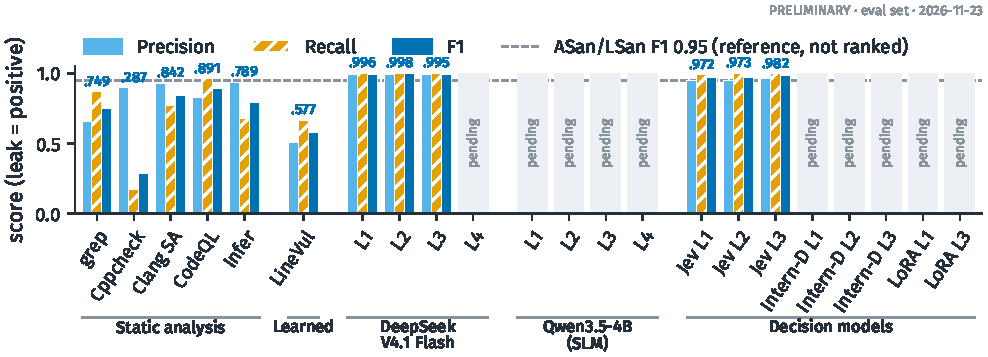
\includegraphics[width=\linewidth,height=0.78\textheight,keepaspectratio]{figures/prf1.pdf}\\[-1pt]
  {\footnotesize Best analyzer CodeQL \res{codeql-layer1}{macro}; DeepSeek L1 \res{deepseek_L1-layer1}{macro}, LoRA L1 \res{lora_L1-layer1}{macro}.
  Juliet is public: layer \ding{174} is the real test.\par}
\end{frame}

% ------------------------------------------------------------------------------
\begin{frame}{Accuracy vs latency: which detector fits which budget?}
  \centering
  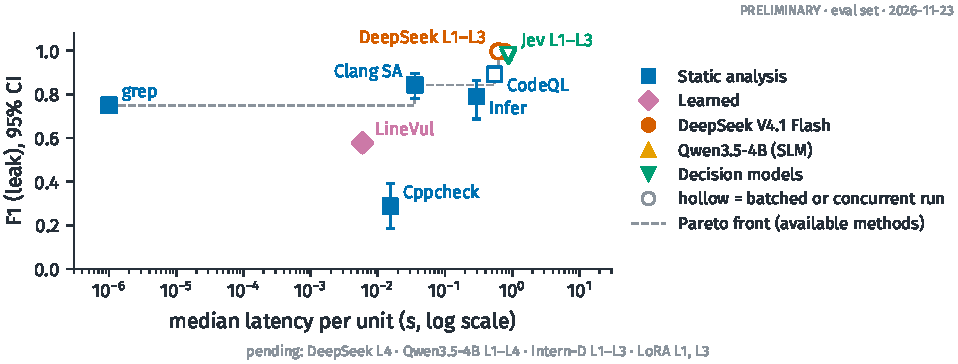
\includegraphics[width=\linewidth,height=0.68\textheight,keepaspectratio]{figures/pareto.pdf}
  \begin{itemize}\small
    \item IDE: Clang SA (18\,ms) or our LoRA (0.1\,s, \res{lora_L1-layer1}{macro}); pre-commit: DeepSeek L1 (0.72\,s)
    \item Latency at concurrency 1 only; CodeQL needs 7.4\,s per unit (0.32\,s amortized over 50)
  \end{itemize}
\end{frame}

% ------------------------------------------------------------------------------
\begin{frame}{Robustness: add a \code{free} that never runs}
  \centering
  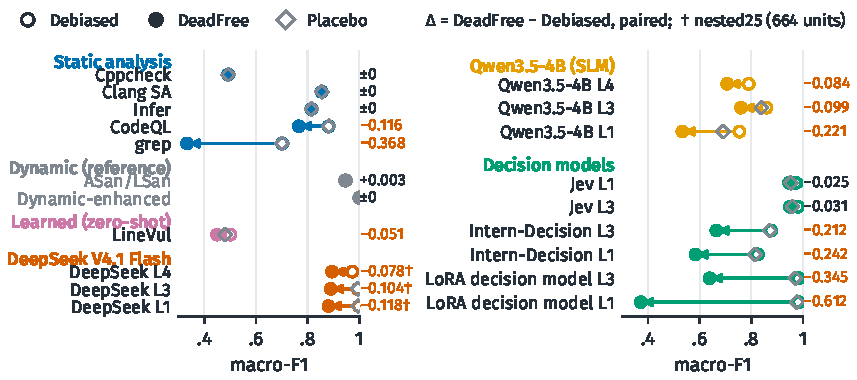
\includegraphics[width=\linewidth,height=0.72\textheight,keepaspectratio]{figures/robustness.pdf}\\[-1pt]
  {\footnotesize Clang SA, Infer: \textbf{0 flips}. \alert{Misses} (trust the dead \code{free}): grep, CodeQL, LoRA.\\
  \alert{False alarms} (doubt a guarded real \code{free}): Qwen, Intern-D. Placebo moves much less.\par}
\end{frame}

% ------------------------------------------------------------------------------
\begin{frame}{Fine-tuning on a shortcut benchmark teaches the shortcut}
  \begin{columns}[c]
    \begin{column}{0.50\textwidth}
      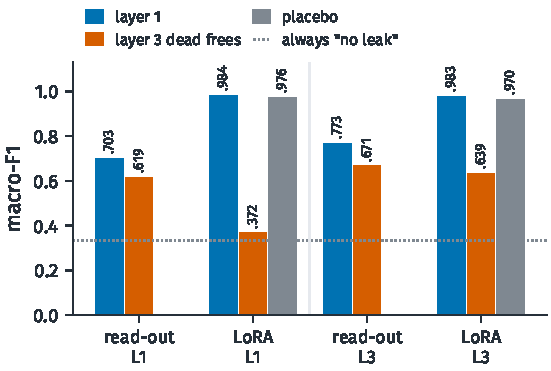
\includegraphics[width=\linewidth]{figures/lora.pdf}
    \end{column}
    \begin{column}{0.48\textwidth}
      \begin{itemize}\small
        \item LoRA L1: \res{lora_L1-layer1}{macro} $\to$ \alert{\res{lora_L1-layer3}{macro}} on layer \ding{174};
              leak recall \alert{\res{lora_L1-layer3}{r}}
        \item Same base, no LoRA: \res{readout_L1-layer1}{macro} $\to$ \res{readout_L1-layer3}{macro}.
              Training sharpened ``\code{free} present $\Rightarrow$ safe''
        \item L3 adds Clang's warnings: \res{lora_L3-layer3}{macro}, recall \res{lora_L3-layer3}{r}.
              Evidence recovers part of the drop
        \item Placebo \res{lora_L1-placebo}{macro}: the cue is the word \code{free}
      \end{itemize}
    \end{column}
  \end{columns}
  \vfill
  {\small Layer \ding{172} accuracy is not evidence of program understanding: test on edits that keep the label.}
\end{frame}

% ------------------------------------------------------------------------------
\begin{frame}[fragile]{L4: LLM facts + Datalog is the most robust prompt}
  \begin{columns}[T]
    \begin{column}{0.56\textwidth}
\begin{lstlisting}[style=dl]
reach("main").
reach(g) :- reach(f), call(f, g, l), !dead(l).
new_obj(o, v, f) :- alloc(o, v, f, l),
                    reach(f), !dead(l).
pts(s, v, o) :- new_obj(o, v, f),
                scope(f, v, s).
pts(sd, d, o) :- assign(d, x, f, l), !dead(l),
                 ..., pts(sx, x, o).
freed(o) :- free(v, f, l), reach(f), !dead(l),
            ..., pts(s, v, o).
(*\textcolor{OIblue}{\bfseries leak(o, "never\_freed")}*) :-
        new_obj(o, _, _), !freed(o).
\end{lstlisting}
      {\tiny Abridged from \texttt{juliet\_full/llm/l4/leak.dl} (v3): Andersen-style, flow-insensitive;
      + \texttt{realloc\_fail} rule.\par}
    \end{column}
    \begin{column}{0.41\textwidth}
      \begin{itemize}\small
        \item DeepSeek L4 on \ding{172}: \res{deepseek_L4-layer1}{macro} (L1 \res{deepseek_L1-layer1}{macro})
        \item On \ding{174}: $\Delta$ \res{deepseek_L4-layer3}{d}, the smallest of L1--L4 (L1 \res{deepseek_L1-layer3}{d})
        \item Errors turn into misses: FP/FN L1 \res{deepseek_L1-layer3}{fp}/\res{deepseek_L1-layer3}{fn},
              L4 \res{deepseek_L4-layer3}{fp}/\res{deepseek_L4-layer3}{fn}
        \item 99.87\% of facts grounded to a source line
        \item Qwen L4: \res{qwen_L4-layer1}{macro}; on \ding{174} \res{qwen_L4-layer3}{macro}
      \end{itemize}
    \end{column}
  \end{columns}
  \vfill
  {\scriptsize Paired on nested25 (664 units). A dead \code{free} is dropped by \code{!dead(l)}, so the leak survives.\par}
\end{frame}
